

%%%%%%
\begin{figure}
\centering
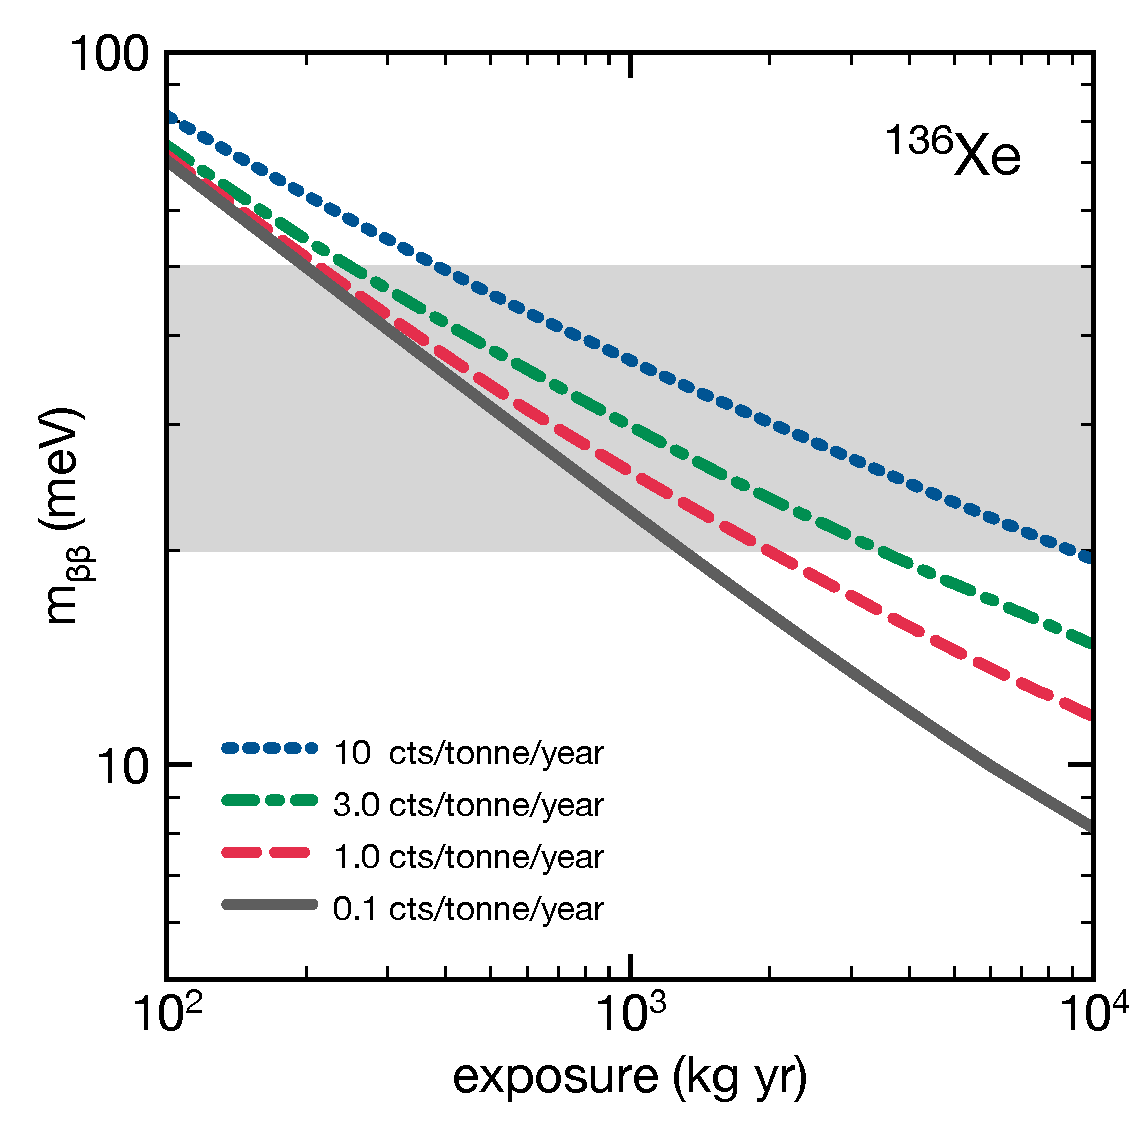
\includegraphics[width=0.90\textwidth]{img2/FutureXe136.pdf}
\caption{\small Sensitivity to \mbb\ as a function of the exposure for different values of the background, for a \XE\ based experiment.} \label{fig.Xe}
\end{figure}
%%%%%%

If no discovery is made by the current generation of experiments, the full exploration of the inverse hierarchy (IH) region (corresponding to \mbb\ values as low as 15~meV) requires detectors of larger mass (at least 1 ton), good resolution and extremely low specific background. In this section we discuss the capabilities of the \HPXE\ technology to explore this scale. 

\subsection{NEXT/NEW as R\&D for a future ton-scale HPXe}

The first goal of the NEXT collaboration during the next three years is to demonstrate, first with NEW, then with NEXT-100, the excellent energy resolution, topological signature and low radioactive budget describe in previous sections. 

It is worth to consider the potential of the HPXe technology using the projected NEXT-100 figures. For a background rate of $6 \times 10^{-4}$ \ckky and an energy resolution of 0.5\% FWHM (e.g, a ROI of 12.5 keV), NEXT would record $\sim$8 events per ton and per year. Naive scaling arguments suggest an improvement of a factor $\sim$2 in the background as the detector dimensions double (and the detector mass multiplies by $\sim$8) to build a ton-scale apparatus. Thus, 4 counts per ton and per year could be expected by a direct extrapolation of the NEXT-100 expected performance. According to Figure \ref{fig.Xe} it would require an exposure of $3 \times 10^{3}~kg\cdot year$, for a 100\% efficient detector, to fully cover the IH. The efficiency of NEXT is around 30\%, and thus, about 10 (5) years of data taking would be necessary to explore the IH for a 1 (2) ton detector which were a direct extrapolation of NEXT-100 (no technological improvement). This qualifies the HPXe technology as a candidate for the ton scale, (since it can cover the IH in a credible time deploying a credible fiducial mass), {\em using existing technology}, provided that NEXT-100 demonstrates both an
energy resolution in the vicinity of 0.5\% FWHM at \Qbb\ and a background rate in the range of 
$5-6 \times 10^{-4}$ \ckky. Thus, NEXT-100, in addition of its physics interest (it can explore a region of effective Majorana masses in the vicinity of $\mbb \sim 100$meV, where a discovery is still possible) can be considered a demonstrator and R\&D apparatus for a ton-scale HPXe-EL.

\subsection{Improving the rejection power of the topological signature}

%%%%%%
\begin{figure}
\centering
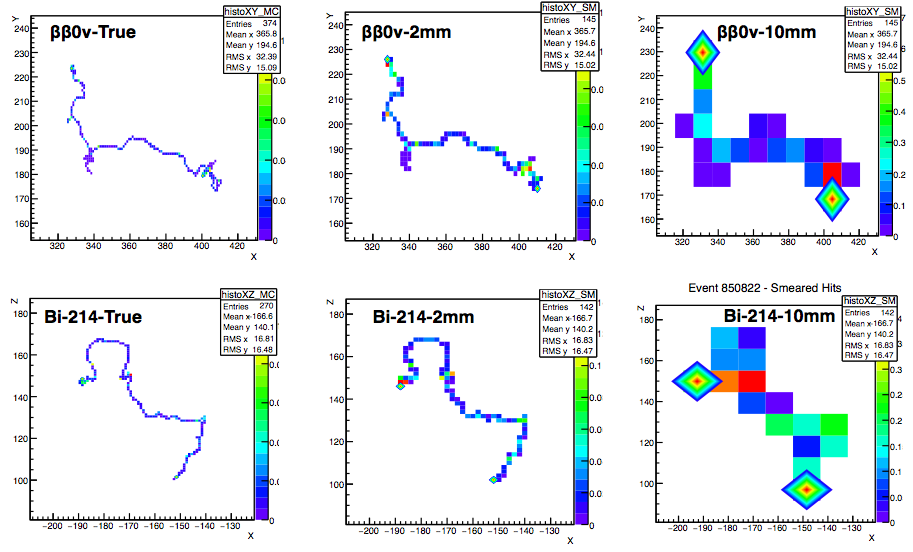
\includegraphics[width=0.90\textwidth]{img2/tracks.png}
\caption{\small Top left: Monte Carlo true hits left by a \bbonu\ event in
an HPXe with no diffusion; top center: hits corresponding to a diffusion of
$2 mm/\sqrt{E}$; top right: hits corresponding to a diffusion of
$10 mm/\sqrt{E}$. Bottom: same, for a single electron produced
by \BI\ decay.} \label{fig.trks}
\end{figure}
%%%%%%

On the other hand, we believe that the performance of an HPXe-EL TPC can improve significantly {\em by improving the topological signature}. 

Currently, the discriminating power of the topological signature is limited by the large diffusion unavoidable in pure xenon. Such large diffusion, of the order of $10 mm/\sqrt{1 m}$, has the effect of blurring the electron(s) trajectory. This, in turn, makes more challenging the task of connecting the hits making up the track and identifying its extremes, where the algorithm searches for the blobs. 

This is illustrated in Figure \ref{fig.trks}. The top panels show a \bbonu\ event, while the bottom panels show a single electron produced by \BI\ decay. From left to right, one can see the true hits of the tracks, and the hits corresponding to a diffusion of $2 mm/\sqrt{E}$~and to a diffusion of
$10 mm/\sqrt{E}$. Notice that in the late case the details of the track are blurred, and in fact, the reconstruction algorithm misidentifies a second blob in the background event, while it succeeds in finding a single blob for the lower diffusion case. 

%%%%%%
\begin{figure}
\centering
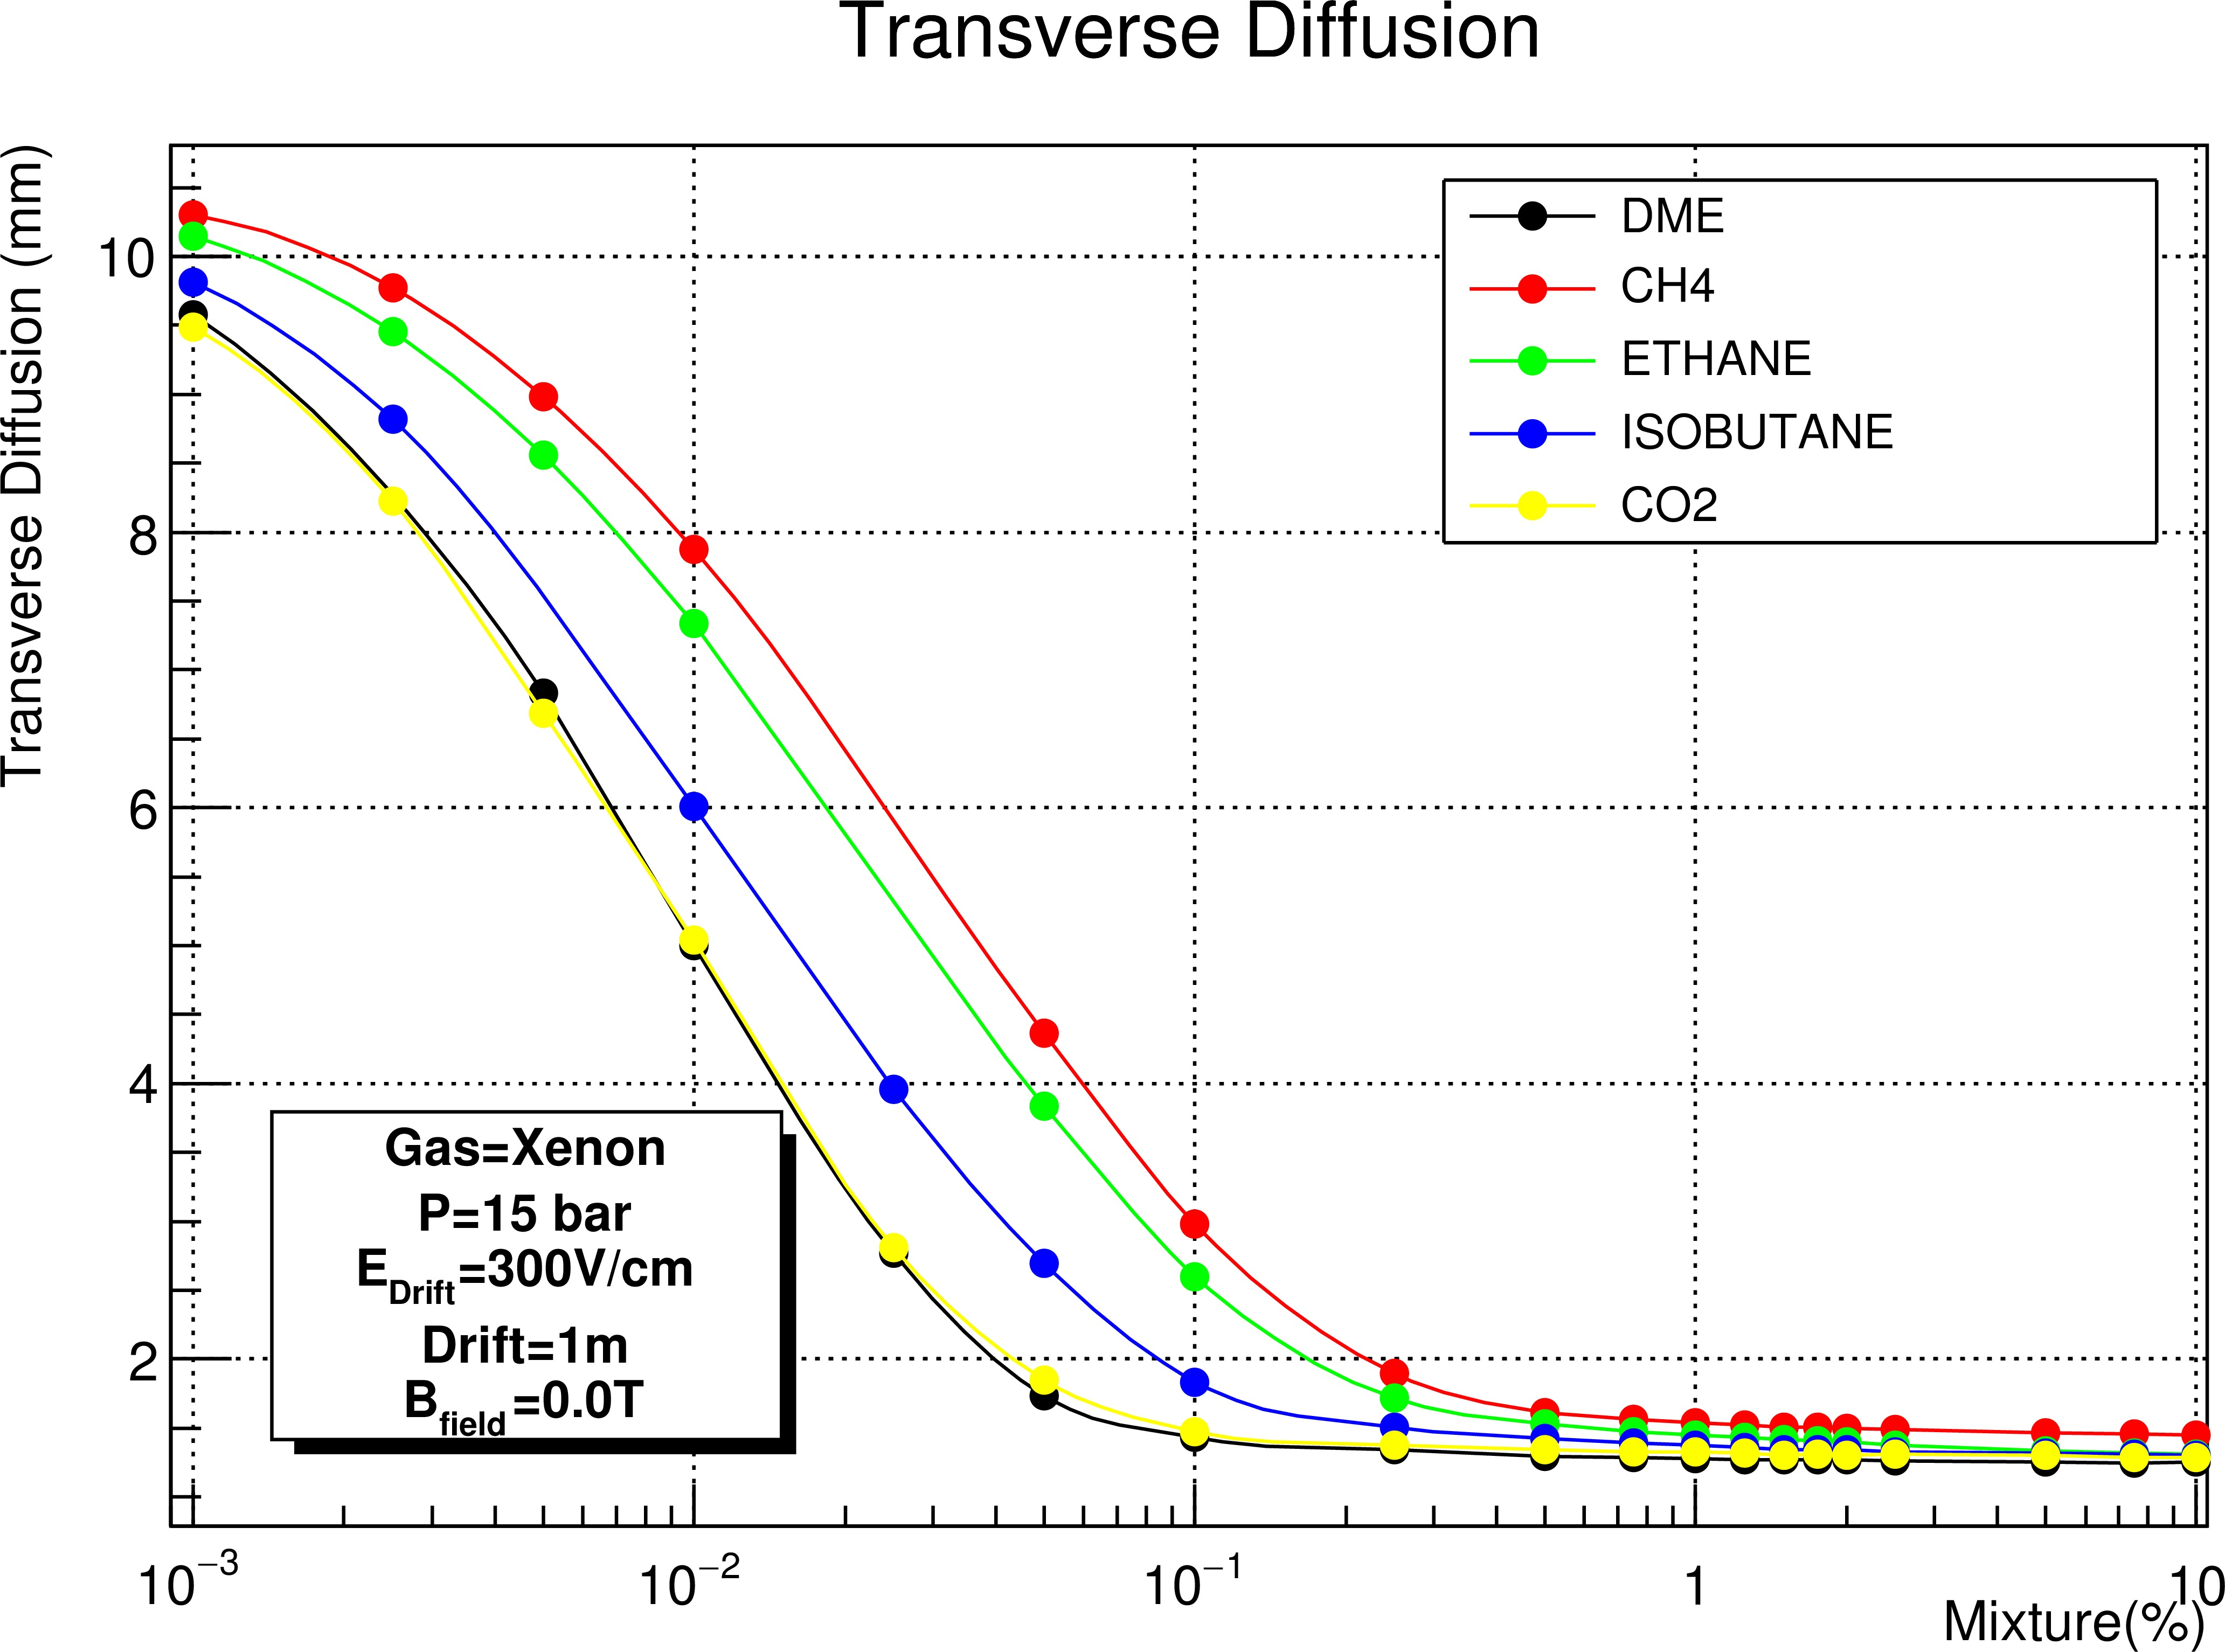
\includegraphics[width=0.90\textwidth]{img2/TD300V.jpg}
\caption{\small Adding small quantities of quencher gases can reduce the diffusion of Xenon to $\sim 1 mm/\sqrt{1 m}$.} \label{fig.QG}
\end{figure}
%%%%%%

%%%%%
%\begin{figure}[!htb]
%	\centering
%	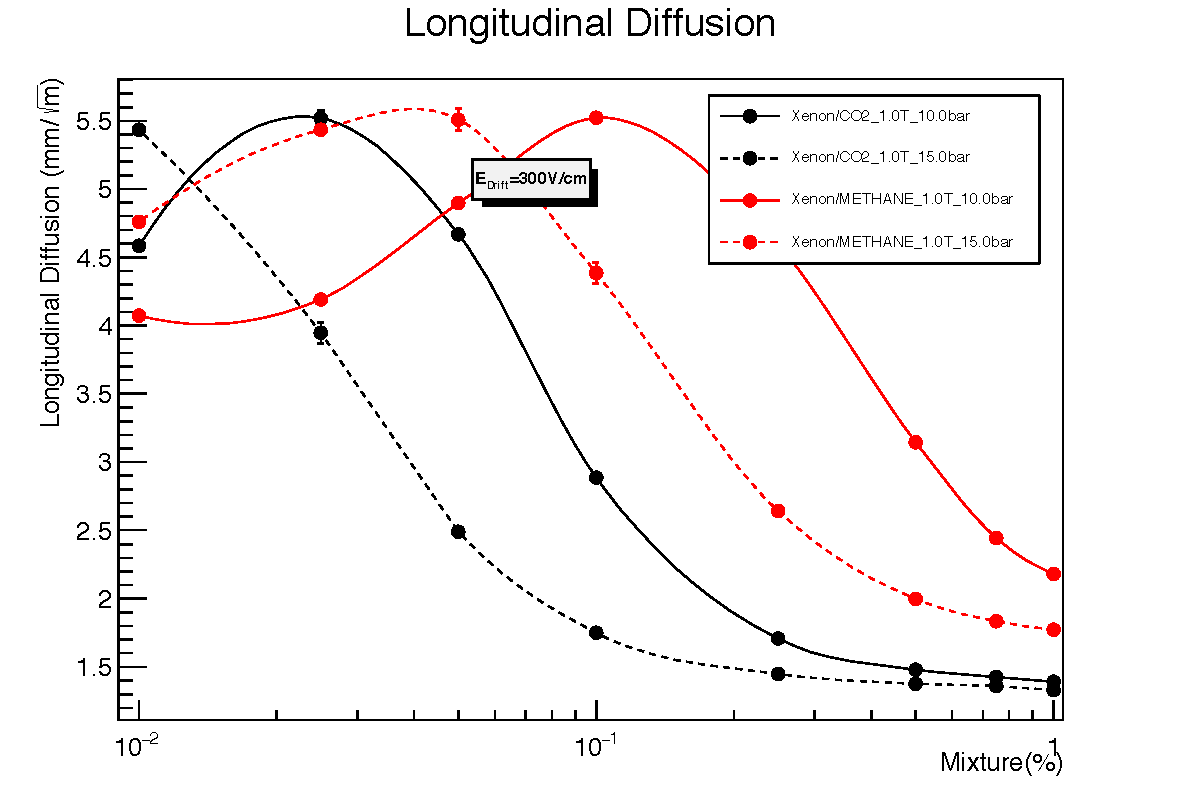
\includegraphics[width=0.75\textwidth]{img/Longitudinal_Diffusion300Vcm.pdf}
%	\includegraphics[width=0.75\textwidth]{img/Transverse_Diffusion300Vcm.pdf}
%	\caption{\label{fig.QG}Longitudinal and transverse diffusion when small amounts of \COT\ and \CHF\ are added to pure xenon. Notice that about 0.3 \% of \COT\ are enough to reduce both longitudinal and transverse diffusion to about $1.5$~mm/$\sqrt{\rm{m}}$.}
%\end{figure}
%%%%%


%%%%%%
\begin{figure}
\centering
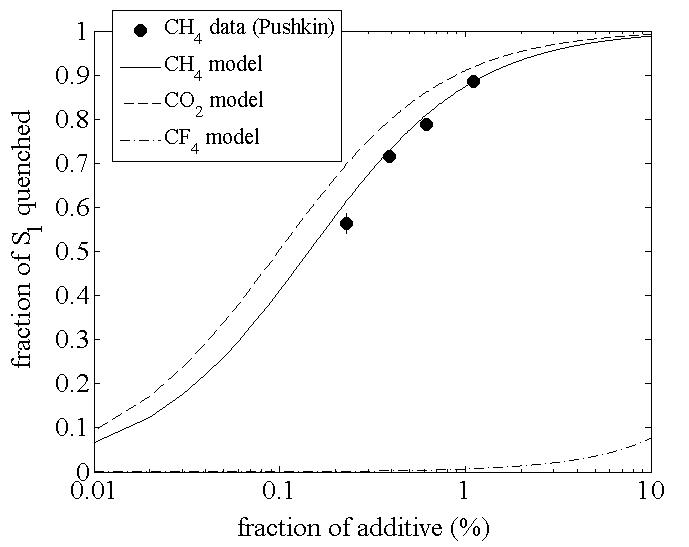
\includegraphics[width=0.90\textwidth]{img2/QF.png}
\caption{\small Adding small quantities of quencher gases also reduces the scintillation light. The plot shows the fraction of S1 light quenched as a function of the fraction of gas added. Notice that a fraction of 0.1\% (0.5\%) of \COT (\CHF) quenches the S1 signal by about 50\% } \label{fig.QF}
\end{figure}
%%%%%%

Diffusion in xenon can be reduced to values as small as 1 mm by adding small amounts of quenching gases, as illustrated in Figure \ref{fig.QG}. On the other hand, quencher gases are known to reduce significantly or even suppress the xenon scintillation light in sufficiently large amounts, as illustrated in Figure \ref{fig.QF}. A major R\&D for the NEXT collaboration during the forthcoming period is to explore the performance of the detector when adding small  mixtures of gases such as \COT\ or \CHF. For example, adding 0.1\% (0.5\%) of \COT (\CHF) would reduce the diffusion to some 2 mm over 1 m of drift, while the predicted quenching of the light would be about 50\%, a factor that appears tolerable and can be partially compensated with higher EL amplification and/or better light collection. 

The R\&D program of NEXT concerning reduction of the diffusion for the next 3 years include:
 \begin{enumerate}
\item {\bf Study of gas mixtures with small setups}. This is already under way, with interesting initial results that suggest that quenching can be smaller than predicted by Monte Carlo calculation. One has to understand carefully, however, the systematics of the measurements. The goal of this studies is to focus in one or two candidates that can be further explored in larger setups. Both \COT\ and \CHF\ appear promising. 
\item {\bf Study of performance in DEMO}. We expect to start the study of selected mixtures (e.g, xenon + 0.1\% \COT, xenon + 0.5\% \CHF) in the NEXT-DEMO detector, late in 2015. DEMO is capable of measuring both S1 and S2 signals, and reconstruct electron tracks, and should provide a quantitative assessment of the effect of the selected mixtures in aspects such as reduction of diffusion, quenching of S1 and S2, attachment, and energy resolution. The goal of the campaign in DEMO is to identify one suitable gas mixture for further studies.
\item {\bf Study of performance in NEW}. Assuming that the previous studies yield promising enough results, the suitable gas mixture candidate(s) will be studied in NEXT during 2017 (2016 will be devote to a run with pure xenon). 
\end{enumerate}

Reducing diffusion to $\sim 2 mm/\sqrt{1 m}$, improves the background rejection of the
HPXE-EL automatically, since the algorithm that finds the blobs at the extremes of the track works much better with the considerable improvement in the hit resolution. Indeed, out Monte Carlo calculations show an improvement of a factor 3-4 in the topological signal rejection factor by simply reducing diffusion to  $\sim 2 mm/\sqrt{1 m}$. This, in turn, translates into 2-3 counts per ton and per year in NEXT-100, and 1-2 counts per ton and per year in a ton scale detector. 
{\em It follows that reducing the diffusion in pure xenon to a target value of 2 mm for 1 m drift while maintaining the energy resolution would permit the exploration of the IH in a short time (e.g, 3 years run) with a HPXE-el of moderate mass (1 ton).}  


\subsection{Adding a magnetic field to enhance the topological signal}
In this section we present a brief status of the on-going studies within the NEXT collaboration to explore the potential of adding a magnetic field to the detector. 

There are two conditions {\em sine qua non}, for a magnetic field to increase the rejection power of an HPXe in a significant way:

\begin{enumerate}
\item The hit resolution must be acceptably low, in the range of 1-3 mm. Thus, a pre-condition for considering the use of a magnetic field is to find a gas mixture providing  low diffusion at an acceptable cost in performance.
\item The track reconstruction must be very efficient finding the extremes of the track and following the track trajectory. This appears possible, for low diffusion (e.g, for a resolution of about 2 mm) using sophisticated pattern recognition algorithms such as minimum spanning trees followed by segment connection.  
\end{enumerate}

When both conditions are fulfilled, it is possible to ``follow'' the track trajectory from one extreme to the other and compute locally quantities such as the track curvature. Notice that the high multiple scattering in dense gas prevents event-by-event measurements of standard variables such as the momentum, or the track curvature. However, one can turn them into statistical estimators, capable of discriminating signal from backgrounds. 

In particular, if the direction of the applied magnetic field is known, the curvature of the track can be calculated to determine whether the component of the electron velocity along the magnetic field is parallel or antiparallel to the field.  Assuming that the magnetic field is directed along the z-axis, we are interested in the curvature of the track in the $x$-$y$ plane as it progresses in $z$.  The curvature $\kappa$ in the $x$-$y$ plane can be calculated for a track parameterized by the coordinate $z$ as

\begin{equation}\label{eqn_curv}
\kappa = \frac{(dx/dz)\cdot(d^2y/dz^2) - (dy/dz)\cdot(d^2x/dz^2)}{\Bigl[(dx/dz)^2 + (dy/dz)^2\Bigr]^{3/2}}.
\end{equation}

With this definition, an electron traveling in the direction of the magnetic field will spiral around the field lines with positive curvature, while an electron traveling opposite the direction of the magnetic field will spiral with negative curvature.  

The curvature, however, will be of the opposite sign if the track orientation is not properly identified in the calculation (i.e., if $dz$ is of the wrong sign).  Thus, when calculating the curvature of a single-electron track, one would expect $\kappa > 0$ for $dz > 0$ and $\kappa < 0$ for $dz < 0$ given that $dz$ is always in the direction of the electron velocity.  However, for a \bbonu\ ``double electron'' (defined as the track between the two blobs that mark the start and end of the trajectory), taking one of the extremes to be the beginning of the track and the other to be the end will lead to a calculation of $\kappa$ assuming the wrong track orientation for one of the two electrons, as the vertex at which the reaction occurred is found somewhere on the interior of the track.  Therefore one expects to find $\kappa > 0$ for $dz < 0$ and $\kappa < 0$ for $dz > 0$ for a significant fraction of the track.  This difference in the behavior of the calculated curvature of reconstructed tracks can be used to distinguish single-electrons from \bbonu\ double electrons.

In the absence of multiple scattering (MS) the transverse momentum of an electron could be directly determined by the track
curvature. Consequently, a single-electron track---for which the momentum is greatest at one end of the track and decreases toward the other end---would be clearly distinguishable
from a double-electron track consisting of two electrons traveling in opposite directions originating at some vertex in the middle of the track.  Unfortunately, in a HPXe TPC multiple scattering is high, resulting in large errors that complicate the direct measurement of the magnitude of the curvature. The sign of the curvature, however, is much less affected by MS (in fact, the gaussian component of MS does not change locally the turning sense of the electron, which is only affected by non-gaussian, large-angle scatters). Consequently we choose the sign of the curvature, rather than its magnitude, as discriminating variable.  

The simplest way to exploit the sign of the curvature is to define a 
curvature asymmetry factor, which simply exploits the fact that signal and background events have different average curvatures (two electrons vs single electron) when turning in the same magnetic field.  A more sophisticated method is to construct a track ``profile'' for each type of event containing the value of the curvature sign at each point along the track averaged over all events.  Since not all tracks will be of exactly the same length, we normalize the track length to 1, and thus the profile contains an average sign value for each fractional distance along the track.  Figure \ref{fig_profiles} shows profiles made for simulated single-electron and $0\nu\beta\beta$ events.  The profiles show a clear separation between signal and background events earlier in the track where the sign of the curvature is most likely to differ.

\begin{figure}[!htb]
	\centering
	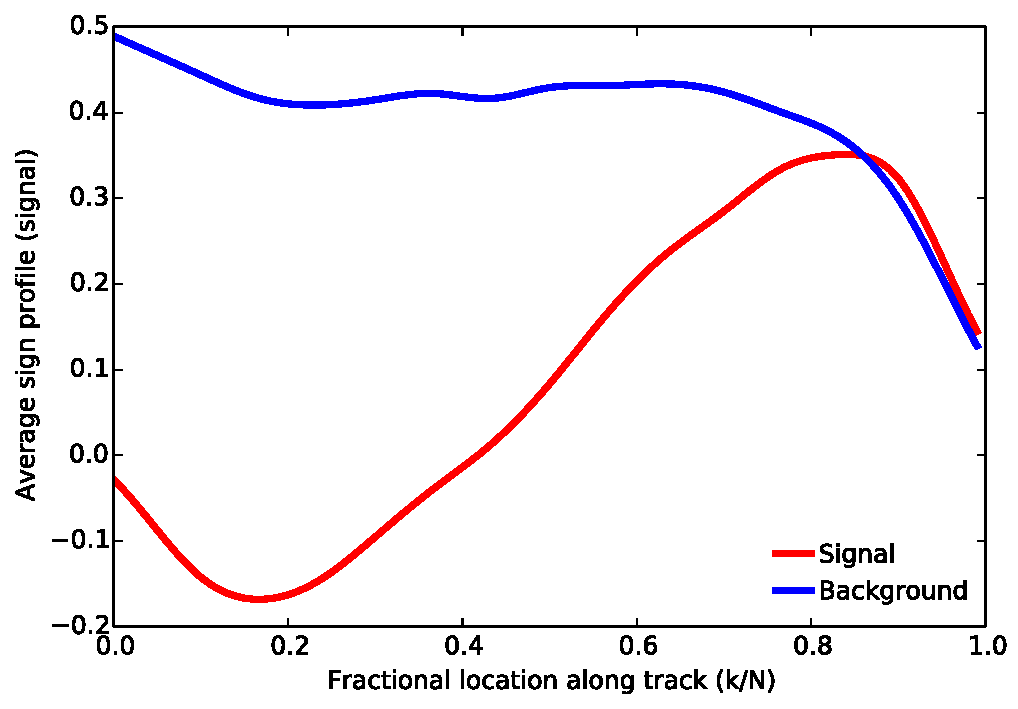
\includegraphics[scale=0.55]{img2/sbprof_nmagse2.pdf}
	\caption{\label{fig_profiles}Average curvature sign profiles for single-electron and $0\nu\beta\beta$ events generated at $B = 0.5$ T and $P = 10$ atm, with $\sigma_{s} = 2$ mm and $N_{s} = 2$.  The profile shows the average sign vs. fractional distance along the track ($k/N$, where $k$ is the hit number and $N$ is the total number of hits).  The profiles were created by dividing the normalized track into 15 bins, and for each calculated curvature value for each event, adding a value of $+1$ or $-1$ to the bin, then dividing each bin by the total number of values placed in it.  The values in the first and second bin were extrapolated linearly to $k/N = 0$, and those in the final two bins were extrapolated to $k/N = 1$.  The entire set of values was then interpolated using cubic polynomials.}
\end{figure}

Once the profiles have been generated, they can be used to define a new variable that will provide separation between the two classes of events.  Figure \ref{fig_svsbprof} compares the signal efficiency obtained for a given background rejection using the profile-based and the method based on the asymmetry factor.  The profile-based method performs better up to a background rejection of about 95\%. Typically a rejection factor of one order of magnitude can be achieved for a signal efficiency of 80\% using the profile method. 

\begin{figure}[!htb]
	\centering
	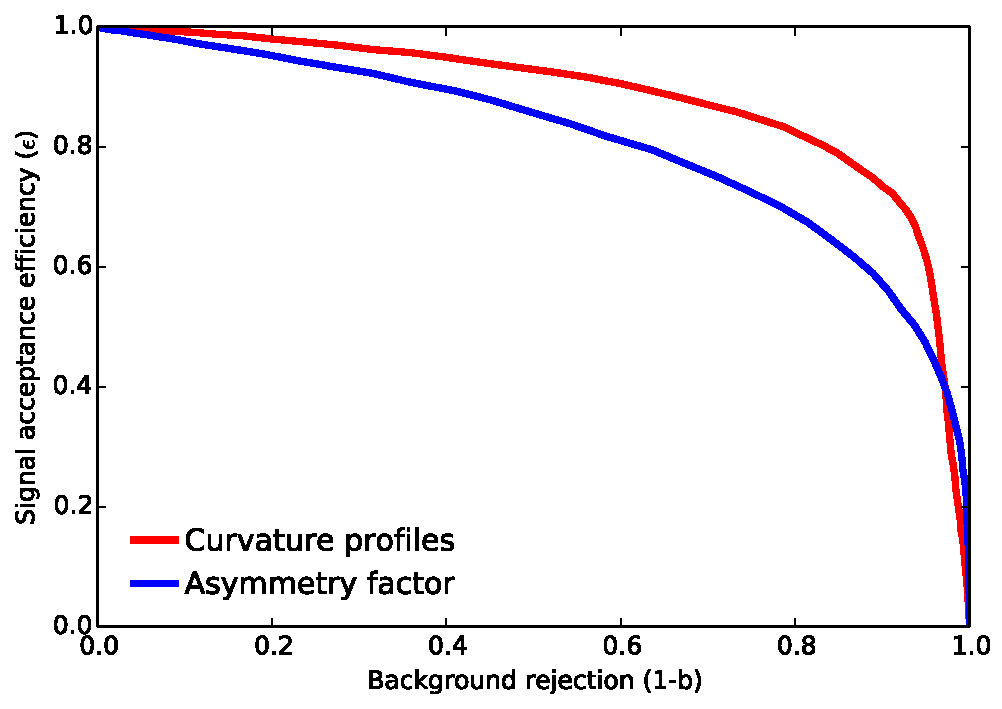
\includegraphics[scale=0.55]{img2/sigvsb_prof_vs_asymm.pdf}
	\caption{\label{fig_svsbprof}Signal acceptance efficiency vs. background rejection obtained at $B = 0.5$ T and $P = 10$ atm, with $\sigma_{s} = 2$ mm and $N_{s} = 2$.  The curve obtained using the curvature asymmetry factor is shown along with that obtained using the profile-based method.}
\end{figure}

The addition of a magnetic field could reduce the background in a ton-scale HPXe well below one count per ton and year, approaching the ``background free'' regime for this scale. On the other hand, the technical difficulties and the costs of adding to the experimental setup a magnet providing a field of around 0.5 Tesla need to be carefully evaluated. 

From the point of view of NEXT R\&D, a test using the NEXT-DEMO detector and the TPC90 magnet, available at CERN (which can run up to 0.7 Tesla) has been approved by the laboratory management. An experimental area has been identified and CERN has agreed to provide the magnet (including water cooling and power) and the infrastructure support. Our schedule foresees to transport NEXT-DEMO and its gas system to CERN in late 2016 and take data in 2017, using several radioactive sources and operating at intensities of 0.1-0.7 Tesla, for about six months.

\subsection{Instrumental upgrades}

There is a number of possible upgrades that could be carried out in a ton-scale HPXe detector with respect to NEXT-100. 

A particularly attractive possibility would be to make the apparatus a symmetric TPC, with the cathode in the center of the field cage and two anodes (+EL grids) in the end-cups. This would permit doubling the detector length with the same electron drift. Indeed, a cylindrical fiducial volume, 2.5 m long and with a diameter of 2.5 m (thus preserving the 1:1 aspect ratio of NEXT-100) would contain a mass of 1060 kg. The fiducial volume would be divided by the cathode in two halves of 1.25 m long (thus slightly more drift than in NEXT-100). Ionisation electrons would drift to one of the two anodes depending on the half of the TPC the event was produced. The EL amplification would be the same design than NEXT-100, doubling the dimensions. The system would consist of a transparent grid, acting as gate and a quartz plate coated with TPB and ITO. The two planes being the anode plates would be identical and would consist of SiPMs of 6 mm and 1 mm located at a pitch of 1 cm. Thus, one would place one SiPM of 1 mm$^2$~followed by 1 SiPM of 6 mm$^2$. The center of the next 1 mm SiPM would be at 1 cm from the previous 1 mm SiPM and the center of the next 6 mm SiPM would be at 1 cm from the previous 6 mm SiPM. This staggered configuration, effectively merges the energy plane and the tracking plane of NEXT-100 in the same multi-function plane. Light is isotropically produced in the EL grid. The light going forward is shift to blue in the anode plate and hits the near-by plane. The small (1 mm) SiPM record the signals used for tracking exactly as in NEXT-100. The signal from the large (6 mm) SiPM is not read, since many of them will be saturated with the intense light, and, in any case, one does not want to measure energy in a plane too near to the light production, to avoid difficult geometrical corrections. Instead, the light going backwards hits either the light tube covering the field cage (and is transferred to blue and part of it reflected towards the far plane) of the anode plate of the far plane, where is shifted to blue and read by the large (6 mm) SiPM. 

The possibility of replacing PMTs by large area SiPMs appears increasingly feasible as the devices have reduced the main source of noise (dark current) by more than one order of magnitude in about 3 years. Currently, the dark current at room temperature is about 70 kHz/mm$^2$, and decreases a factor 2 every time that the temperature decreases 10 degrees. Cooling the tracking planes to $\sim$ -10 degrees C appears reasonable and would decrease the dark current to less than 10 kHz/mm$^2$. Our Monte Carlo simulations indicate that a performance comparable with that of PMTs can be obtained for dark currents below
50 kHz/mm$^2$.  

A symmetric TPC readout exclusively by SiPMs would represent a considerable improvement with respect to NEXT-100, both in terms of the increase in size (while keeping the same drift length), the radio purity and the simplicity of the design. The use of SiPMs would eliminate the need for PMTs which are one of the driving sources of background in NEXT-100 (instead, the SiPMs currently used by NEXT-100 are measured to be extremely radiopure) and also the need for the complex vacuum-enclosure system. Last but not least, such a SiPM-only apparatus could operate in a magnetic field. 

\subsection{A ton scale HPXe experiment: cost estimate}

\begin{table}[htdp!]
\caption{Cost estimate for a ton-scale HPXe-EL TPC}
\begin{center}
\begin{tabular}{|l|l|l|l|l|}
\hline
Item	& unit cost & number of units &	Total cost	(M\$)\\
\hline
\XE\ & 15 \$/g & $10^6$ & 15 \\
SiPM tracking & 7 & $10^5$ & 0.7 \\
SiPM energy & 15 & $10^5$ & 1.5 \\
FEE + DAQ & 15 & $2 \times 10^5$ & 3 \\
Gas system & 0.8 & 1 & 0.8 \\
Water tank & 1.0 & 1 & 1.0 \\
Mechanics & 1.0 & 1 & 1.0 \\
Shielding & 1.0 & 1 & 1.0 \\
\hline
Total & & & 24 \\
\hline
\hline
\end{tabular}
\end{center}
\label{tab.costs}
\end{table}%


The cost of a future ton-scale HPXe-EL detector would be dominated by the cost of the \XE. The cost of the enriched xenon for NEXT-100 was about 10 \$ per gram but we quote here a conservative estimate of 15 \$ per gram, resulting in about 15 M\$ for one ton. The next elements driving the cost are the SiPMs. One needs 10$^5$~1 mm SiPMs and 10$^5$~6 mm
SiPMs (50,000 per plane). A conservative estimate (at today's prices and correcting for the larger order) is 7 \$ per unit for the 1 mm parts and 15 \$ per unit for the 6 mm parts. The cost of the front-end electronics and DAQ in NEXT-100 was 15\$ per channel. The same electronics can be used for the ton scale. The cost of the gas system for NEXT-100 is about 0.4 M\$, thus 0.8 M\$ appears reasonable for the larger system. Adding 1M\$ for the water tank, 2M\$ for mechanics (including pressure vessel, field cage anode plates, etc), and 1 M\$ for ultra pure copper shielding (internal to the vessel) adds to 24 M\$. The costs are summarised in Table \ref{tab.costs}. 

